\scanpage{36}
\begingroup
\setlength{\tabcolsep}{0pt}
\setbox0=\hbox{%
\begin{tabular}{@{}l@{\hspace{1em}}l@{\hspace{1em}}l@{}}
\parbox[t][21em][t]{30em}{%
\(H^0(X,\zeta_\ell)=U_\ell\)\par\vspace{3em}
\(\begin{aligned}
H^2(X,\mathbb Z/\ell)&=H^2(X,\zeta_\ell)\otimes_{\mathbb Z/\ell}\operatorname{Hom}(U_\ell,\mathbb Z/\ell)\\[1em]
&=\unsure{\mathbb Z|\zeta}_\ell\otimes_{\mathbb Z/\ell}\operatorname{Hom}(U_\ell,\mathbb Z/\ell)\\[1em]
&\simeq\deleted{\mathbb Z/\ell}\operatorname{Hom}(U_\ell,\mathbb Z/\ell)
\end{aligned}\)}
&
\parbox[t][21em][t]{40em}{%
\(H^1(X,\zeta_\ell)=P^{(\ell)}\)\quad\unsure{élémts|élts} de la jacobienne\par
\hspace*{15em}$P$ de $X$\unsure{,|.} annulés par $\ell$\par\vspace{2.3em}
\(\begin{aligned}
H^1(X,\mathbb Z/\ell)&=H^1(X,\zeta_\ell)\otimes_{\mathbb Z/\ell}\operatorname{Hom}(\unsure{U|\zeta}_\ell,\mathbb Z/\ell)\\[.6em]
&\deleted{=P^{(\ell)}\otimes}\quad\overset{\text{''}\quad}{\deleted{\operatorname{Hom}(\zeta_\ell,H}}\\[.6em]
&=P^{(\ell)}\otimes_{\mathbb Z/\ell}\operatorname{Hom}(\unsure{U|\zeta}_\ell,\mathbb Z/\ell)
\end{aligned}\)\par\vspace{1em}
\hspace*{3em}Or\quad\(P^{(\ell)}\times P^{(\ell)}\longrightarrow U_\ell\)\quad\unsure{en vertu}\par\vspace{.5em}
\hspace*{6em}%
\begingroup
\setbox2=\hbox{\strut de\hspace{1.4em}\begin{tabular}[t]{@{}l@{}}
l'autodualité de $P$ \textendash\,\textendash\,\textendash\\
\uline{et} la dualité de Kummer-Serre \textendash
\end{tabular}\hspace{.5em}}
\dimen2=\dimexpr\ht2+\dp2\relax
\rlap{\raisebox{-\dp2}{\begin{tikzpicture}[x=\wd2,y=\dimen2,baseline=0pt]
\useasboundingbox (0,0) rectangle (1,1);
\draw[line width=.3pt] (.135,1.09) .. controls (.42,1.16) and (.82,1.13) .. (.98,1.07) -- (.995,1.00);
\draw[line width=.3pt] (.12,.94) -- (.125,-.10);
\draw[line width=.3pt] (-.01,.79) -- (-.005,-.05) -- (.125,-.10) .. controls (.53,-.07) and (.82,-.03) .. (.99,-.02);
\draw[line width=.3pt] (1.00,.77) -- (1.00,.08);
\end{tikzpicture}}}\box2
\endgroup}
&
\parbox[t][21em][t]{27em}{%
\(H^2(X,\zeta_\ell)\simeq\mathbb Z/\ell\)\par\vspace{3.3em}
\(H^0(X,\mathbb Z/\ell)\simeq\mathbb Z/\ell\)}
\\
\parbox[t][12.8em][t]{30em}{%
\vspace*{1em}\(H^0(X,\zeta_p)=0\)\par\vspace{3em}
\(H^2(X,\mathbb Z/p)\simeq H^2(X,\mathbb Z/p)\simeq0\)}
&
\parbox[t][12.8em][t]{40em}{%
\vspace*{1em}\hspace*{3.5em}\(H^1(X,\zeta_p)=P^{(p)}\ =\)\quad\unsure{élémts|élts} d'ordre $p$\par
\hspace*{16em}de la jacobienne\par\vspace{1.8em}
\hspace*{3.5em}\(H^1(X,\mathbb Z/p)\simeq\)\unsure{élémts|élts} de \(H^1(X,\underline{\mathrm O}_X)\) fixes\par
\hspace*{23em}par $F$\par\vspace{.7em}
\hspace*{7em}%
\begingroup
\setbox2=\hbox{\hspace{.6em}\strut dualité de Serre - Cartier\hspace{.6em}}
\dimen2=\dimexpr\ht2+\dp2\relax
\rlap{\raisebox{-\dp2}{\begin{tikzpicture}[x=\wd2,y=\dimen2,baseline=0pt]
\useasboundingbox (0,0) rectangle (1,1);
\draw[line width=.3pt] (.025,1.27) -- (.17,1.25);
\draw[line width=.3pt] (.185,1.25) .. controls (.50,1.23) and (.80,1.32) .. (1.00,1.36);
\draw[line width=.3pt] (0,1.02) -- (0,-.23) .. controls (.25,-.28) and (.75,-.13) .. (1.00,-.11);
\draw[line width=.3pt] (1.00,1.08) -- (1.00,.02);
\end{tikzpicture}}}\box2
\endgroup}
&
\parbox[t][12.8em][t]{27em}{%
\vspace*{.6em}\(H^2(X,\zeta_p)\simeq\mathbb Z/p\)\par\vspace{3.5em}
\(H^0(X,\mathbb Z/p)\simeq\mathbb Z/p\)}
\\
\parbox[t][5.4em][t]{30em}{\vspace*{1.3em}\(H^0(X,i_p)=0\)}
&
\parbox[t][5.4em][t]{40em}{\vspace*{1.3em}\hspace*{8em}%
\(H^1(X,\unsure{i}_p)\simeq{}_F H^1(X,\underline{\mathrm O}_X)\)%
\raisebox{1.7ex}{
\begin{tikzpicture}[x=.25ex,y=.25ex]\fill (0,3)--(1.2,4.2)--(2.8,5.1)--(4.2,5)--(4.8,4.6)--(6.4,5.3)--(6.5,4.6)--(5.6,3.8)--(5.9,2.8)--(5.2,1.5)--(3.7,0)--(3.3,.8)--(2.8,.1)--(2.2,.8)--(1.1,.7)--(1.2,2.7)--cycle;\end{tikzpicture}}}
&
\parbox[t][5.4em][t]{27em}{\vspace*{1.3em}\(H^2(X,i_p)=H^1(X,\underline{\mathrm O}_X)_F\)}
\end{tabular}}
\dimen0=\dimexpr\ht0+\dp0\relax
\noindent\resizebox{\linewidth}{!}{\hspace*{15em}%
\llap{\raisebox{\dimexpr.45\dimen0-\dp0\relax}{\rotatebox{90}{Cohomologie discrète}}\hspace{12.7em}}%
\llap{\raisebox{\dimexpr.37\dimen0-\dp0\relax}{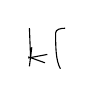
\begin{tikzpicture}[x=1ex,y=1ex]\draw (0.8,4)--(0.9,1.5); \draw (0.7,1.5)--(2.3,1.8); \draw (1,2.4)--(0.8,0.8); \draw (0.7,1.6)--(2.1,1.1); \draw (3.8,4)..controls (3.4,4) and (3,3.9)..(3,3.6)..controls (3,2.5) and (3,1.3)..(3.4,0.6);\end{tikzpicture}}\hspace{12.7em}}%
\rlap{\raisebox{-\dp0}{\begin{tikzpicture}[x=\wd0,y=\dimen0,baseline=0pt]
\useasboundingbox (0,0) rectangle (1,1);
\draw[line width=.3pt] (.307,1.025) .. controls (.305,.83) and (.308,.67) .. (.309,.48) -- (.310,.425);
\draw[line width=.3pt] (.310,.419) -- (.312,.285);
\draw[line width=.3pt] (.312,.279) -- (.312,.14) .. controls (.312,.08) and (.315,.02) .. (.318,-.025);
\draw[line width=.3pt] (.720,1.025) .. controls (.723,.82) and (.720,.65) .. (.722,.523);
\draw[line width=.3pt] (.724,.520) .. controls (.722,.51) and (.725,.50) .. (.724,.480);
\draw[line width=.3pt] (.725,.464) .. controls (.727,.42) and (.723,.38) .. (.726,.350)
-- (.728,.343) -- (.725,.337) .. controls (.727,.30) and (.727,.28) .. (.725,.267)
.. controls (.724,.256) and (.727,.253) .. (.726,.246)
.. controls (.729,.21) and (.729,.17) .. (.726,.14)
.. controls (.724,.11) and (.726,.09) .. (.730,.09) -- (.733,.086) -- (.731,.080)
.. controls (.728,.05) and (.731,.015) .. (.734,-.025);
\draw[line width=.3pt] (.729,-.270)--(.735,-.282);
\draw[line width=.3pt] (-.12,.464) .. controls (.20,.463) and (.52,.471) .. (.72,.462) .. controls (.86,.459) and (.98,.462) .. (1.01,.474);
\draw[line width=.3pt] (-.12,.138) .. controls (.06,.137) and (.23,.142) .. (.305,.141);
\draw[line width=.3pt] (.322,.141) .. controls (.51,.147) and (.63,.142) .. (.72,.139) .. controls (.88,.139) and (.98,.142) .. (1.01,.139);
\draw[line width=.3pt] (-.075,.925) .. controls (-.085,.93) and (-.086,.79) .. (-.082,.65)
.. controls (-.078,.57) and (-.093,.515) .. (-.112,.50)
.. controls (-.087,.478) and (-.078,.44) .. (-.079,.35)
.. controls (-.083,.25) and (-.086,.18) .. (-.075,.155);
\end{tikzpicture}}}\box0}
\endgroup
\margin{35}
